\documentclass[a4paper, 12pt]{article}
\usepackage[utf8]{inputenc}  % Unicode
\usepackage[french]{babel}
\usepackage{geometry}
\usepackage{graphics}
\usepackage[pdftex]{graphicx, color}
\usepackage{pdfpages}
\DeclareGraphicsExtensions{.jpg,.png}
\pdfoutput=1
\usepackage[pdftex,
	bookmarks = true,           % Signets
	bookmarksnumbered = true,   % Signets numerotes
	pdfstartview = FitV,        % La page prend toute la hauteur
	colorlinks=true,
	citecolor=black,urlcolor=blue,linkcolor=black,
	pdfauthor={Auteur},
	pdftitle={Titre},
 	pdfsubject={Sujet},
%	pdfkeywords={},	% Besoin de keywords ?
	plainpages=false,
	pdfpagelabels,
	breaklinks=true,
   	hyperindex,
	linktocpage=true	% pour colorier seulement le numéros dans la TOC	
]{hyperref}
\usepackage{float}
\usepackage{listings}
\usepackage{alltt}
\renewcommand{\ttdefault}{txtt}

\lstset{basicstyle=\ttfamily,
escapeinside={||},
mathescape=true}
\setcounter{secnumdepth}{3}
\newcommand{\HRule}{\rule{\linewidth}{0.5mm}}

\newcommand*\styleC{\fontsize{9}{10pt}\selectfont }
\newcommand*\styleD{\fontsize{9}{10pt}\usefont{OT1}{pag}{m}{n}\selectfont }

\makeatletter
% on fixe le langage utilisé
\lstset{language=matlab}
\edef\Motscle{emph={\lst@keywords}}
\expandafter\lstset\expandafter{
}
\makeatother



\definecolor{Ggris}{rgb}{0.45,0.48,0.45}

\lstset{emphstyle=\ttfamily\color{blue}, % les mots réservés de matlab en bleu
basicstyle=\ttfamily\styleC, % 
keywordstyle=\ttfamily,
commentstyle=\color{Ggris}\styleD, % \styleD commentaire en gris
numberstyle=\tiny\color{black},
numbers=left,
numbersep=10pt,
lineskip=0.7pt,
showstringspaces=false}
%  % inclure le fichier source
\newcommand{\FSource}[1]{%
\lstinputlisting[texcl=true]{#1}
}

%%%%%%%%%
\textwidth=15cm
\textheight=21cm
%\hoffset=-2.5cm
\tolerance=9000
\hbadness=9000
\pretolerance=2500


\begin{document}
%\rmfamily

\begin{titlepage}
\begin{center}



\textsc{\Large Rapport de TP - SY26}\\[0.5cm]
\vspace{4cm}
% Title
\HRule \\[0.4cm]
{ \huge \bfseries TP02 - Codage de Huffman \\[0.4cm] }

\HRule \\[1.5cm]

% Author and supervisor
\begin{minipage}{0.4\textwidth}
\begin{flushleft} \large
R\'emi \textsc{Burtin}
\end{flushleft}
\end{minipage}
\begin{minipage}{0.4\textwidth}
\begin{flushright} \large
Cyril \textsc{Fougeray}
\end{flushright}
\end{minipage}

\vspace{4cm}

{\large \today}



\vfill
% Bottom

\includegraphics[width=0.25\textwidth]{logo.jpg}\\[0.5cm]

\textsc{\LARGE Universit\'{e} de Technologie de Compi\`{e}gne}\\[1.5cm]


\end{center}
\end{titlepage}


%\begin{abstract} 
%\end{abstract} 

%{\bf Keywords:} \newline


\clearpage

\section{Introduction}
L'objectif de ce TP est de programmer l'algorithme itératif de Lloyd-Max pour la conception d'un quantificateur scalaire optimal.

\section{Quantification uniforme}

\subsection{Distorsion normalisée et rapport signal bruit}\label{dist_nmse_snr}

Ce premier script nous permet de calculer la distorsion normalisée (NMSE) ainsi que le rapport signal/bruit (Signal to Noise Ratio - SNR).

Pour cela, nous utilisons la fonction \textit{lloyds} qui permet d'encoder un vecteur (ici une image en vecteur ligne) selon Lloyd-Max avec un nombre précis de partitions (correspondant aux nombre de valeurs de reconstruction). Cette fonction \textit{lloyds} retourne la distorsion (non normalisée). Afin de calculer la distorsion normalisée, nous devons diviser cette distorsion $D$ par la variance du vecteur passé à la fonction :
		\[NMSE = \frac{D}{\sigma_X^2} 
	\]


\subsubsection{R\'esultats}
\label{sec:Resultats}

Après avoir exécuté la fonction, nous nous rendons compte des résultats : 

\begin{alltt}
>> [nmse snr] = disto_1_1('lena.bmp', \textbf{2})
nmse = 0.3009
snr = 5.2157

>> [nmse snr] = disto_1_1('lena.bmp', \textbf{8})
nmse = 0.0190
snr = 17.2149

>> [nmse snr] = disto_1_1('lena.bmp', \textbf{256})
nmse = 0
snr = Inf
\end{alltt}

Lors de la première exécution, nous choisissons d'encoder l'image avec 2 valeurs différentes (correspondant à 2 niveaux de gris dans notre cas). La distorsion est donc importante, et maximale (il n'est pas possible et inutile d'encoder l'image avec 1 seule valeur car aucune information n'est conservée dans ce cas).

Évidemment, dans le cas où nous encodons l'image avec 256 niveaux de gris (telle que l'image originale), aucune distorsion n'est présente.


\subsection{Quantification uniforme}
\label{sec:quantif_uniforme}

Nous allons maintenant programmer une fonction permettant la quantification uniforme d'une image à partir d'un débit, correspondant aux nombre valeurs de reconstruction. Cette fonction renvoie l'image quantifiée ainsi que la distorsion avec l'image originale. \\

L'image originale utilisée sera ici en niveau de gris. Si l'image passée en paramètre de la fonction est une image en couleur, elle sera alors convertie via la fonction \textit{rgb2gray}. Le signal $X$ obtenu est alors borné entre la valeur minimum 0 et la valeur maximum 255 (domaine de variation). \\

Nous allons utiliser la fonction \textit{quantiz} afin de quantifier uniformément l'image. Cette fonction permet de choisir les seuils de décision ainsi que les valeurs de reconstruction pour un signal donné.\\

Pour quantifier uniformément le signal, nous allons construire $N$ niveaux de reconstruction ce qui nous permettra de définir nos seuils de décision. $N$ est ici fonction du débit binaire $R$ passé en paramètre de la fonction de quantification : $N=2^R$. Ainsi, nous devons construire $N+1$ seuils de décision. Afin de partitionner uniformément le domaine de variation, nous utilisons la fonction \textit{linspace} qui permet de créer un vecteur ayant des valeurs linéairement réparties entre une borne inférieure et une borne supérieure. La fonction \textit{quantiz} nous impose la suppression de ces bornes dans le vecteur des seuils de décision, comme énoncé dans la documentation de la fonction : 
\begin{alltt}
 Elements of INDX = 0, 1, 2, ..., N-1 represent SIG in the range of 
[\textbf{-Inf, PARTITION(1)}], [PARTITION(1), PARTITION(2)], [PARTITION(2), 
PARTITION(3)], ..., [\textbf{PARTITION(N-1), Inf}].
\end{alltt}
Ainsi, les deux bornes extrêmes seront automatiquement $-\infty$ et $+\infty$. La fonction \textit{linspace} a inclus les bornes dans le vecteur, nous devons donc supprimer les valeurs 0 et 255 de notre vecteur \verb+PARTITION+. \\

Nous devons maintenant choisir nos valeurs de reconstruction $r_i, i\in[1, N]$. Lors d'une quantification uniforme, ces valeurs de reconstruction sont au milieu des seuils de décisions, soit la moyenne des seuils de décisions consécutifs : $r_i = (d_i + d_{i+1})/2$. Une boucle permet de construire un vecteur contenant les valeurs de reconstruction à partir du vecteur des seuils de reconstruction (\textit{cf} Annexe \ref{quant_uni_code}). L'image quantifiée est donc retournée par la fonction \textit{quantiz}, nous la reconstruisons ensuite afin d'obtenir une matrice, telle que l'image originale. Afin d'afficher l'image via la fonction \textit{imshow}, il faut diviser les valeurs de la matrice par 255. \\

Nous exécutons la fonction dans MATLAB : 
\begin{verbatim}
[image_quant dist] = quant_uni_1_2('lena.bmp', 2);
partition =
   63.7500  127.5000  191.2500
codebook =
   31.8750   95.6250  159.3750  223.1250
>> imshow(image_quant./255)
>> dist
dist = 331.5913
\end{verbatim}

\begin{figure}[H]
	\centering
		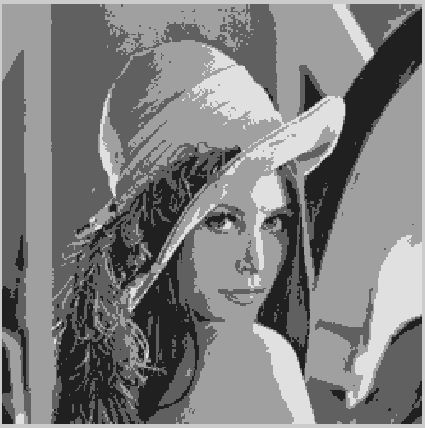
\includegraphics[width=6cm, height=6cm]{../lena_quant_4_niveaux.jpg}
	\caption{Quantification uniforme, lena.bmp, débit = 2}
	\label{fig:lena_quant_4_niveaux}
\end{figure}

Les valeurs de reconstruction sont au milieu de chaque intervalle. Ces intervalles sont répartis entre 0 et 255 ce qui implique qu'il est impossible de retrouver les valeurs de reconstruction 0 ou 255. La distorsion est donc dans tous les cas non nulle dans notre cas. \\

\subsection{Tests sur les différentes images}

\begin{table}[H]
	\centering
		\begin{tabular}{l|c|c|c|}
			\cline{2-4}
			                               & 4 niveaux & 8 niveaux & 64 niveaux \\
			\hline
			\multicolumn{1}{|l|}{Lena}     & 331.59    &  83.38    & 1.28       \\
			\hline
			\multicolumn{1}{|l|}{Peppers}  & 309.10    &  86.97    & 1.29       \\
			\hline
			\multicolumn{1}{|l|}{Harbour}  & 282.88    &  113.16   & 1.21       \\
			\hline
			\multicolumn{1}{|l|}{Bridge}   & 331.21    &  84.13    & 0.87       \\
			\hline
			\multicolumn{1}{|l|}{Boats}    & 226.24    &  92.48    & 1.28       \\
			\hline
			\multicolumn{1}{|l|}{Airfield} & 405.28    &  92.13    & 1.37       \\
			\hline
		\end{tabular}
	\caption{Comparaison des distorsions}
	\label{tab:TableComparaisonDistoUniforme}
\end{table}

\subsection{Huffman - Taux de compression des images quantifiées}


\begin{table}[H]
	\centering
		\begin{tabular}{l|c|c|c|}
			\cline{2-4}
			                               & Uniforme 4 niveaux & Uniforme 16 niveaux       & Sans      \\
			\hline
			\multicolumn{1}{|l|}{Lena}     & 77.08 \%           & 55.66 \%                  & 6.66 \%   \\
			\hline
			\multicolumn{1}{|l|}{Peppers}  & 77.05 \%           & 53.82 \%                  & 4.77 \%   \\
			\hline
			\multicolumn{1}{|l|}{Harbour}  & 79.56 \%           & 59.86 \%                  & 15.21 \%  \\
			\hline
			\multicolumn{1}{|l|}{Bridge}   & 77.27 \%           & 53.14 \%                  & 28.35 \%  \\
			\hline
			\multicolumn{1}{|l|}{Boats}    & 80.6 \%            & 60.80 \%                  & 11.74 \%  \\
			\hline
			\multicolumn{1}{|l|}{Airfield} & 75.31 \%           & 52.46 \%                  & 10.70 \%  \\
			\hline
		\end{tabular}
	\caption{Taux de compression avec Huffman}
	\label{tab:TableComparaisonTauxCompressionUniforme}
\end{table}

\section{Quantification scalaire optimale de Lloyd-Max}

\subsection{Mise en oeuvre}

La programmation de la fonction de quantification scalaire optimale de Lloyd-Max se fait à l'aide de deux paramètres : le signal (dans notre cas une image), et le débit disponible (bits/pixel). Cette fonction renvoie l'image quantifiée. \\

Pour initialiser l'algorithme, nous utilisons une simple quantification uniforme. Ensuite, nous allons chercher à minimiser l'erreur quadratique à l'aide d'une boucle itérative. A chaque itération, il faut que la valeur de reconstruction se rapproche de la moyenne des échantillons dans un intervalle donné : application de la condition du centroïde. A noter que, comme indiqué dans l'énoncé, lorsque l'intervalle est vide, la valeur de reconstruction devient le centre de l'intervalle. Ensuite, nous modifions l'intervalle (valeurs de décision) en appliquant la règle du plus proche voisin. L'image est quantifiée à l'aide des valeurs de reconstruction et des seuils de décisions via la fonction \textit{quantiz} (vue dans la partie précédente). Sa distorsion est recalculée et comparer à la précédente à chaque itération ce qui permet de sortir de la boucle lorsque cette distorsion ne fluctue plus beaucoup. La condition d'arrêt que nous avons fixé est une différence de distorsion inférieur à $0.1$. Lorsque la distorsion se stabilise, nous reconstruisons l'image afin de pouvoir l'afficher ensuite. L'ensemble de l'algorithme est disponible en annexe \ref{quant_lloyd}\\

\begin{figure}[H]
	\centering
		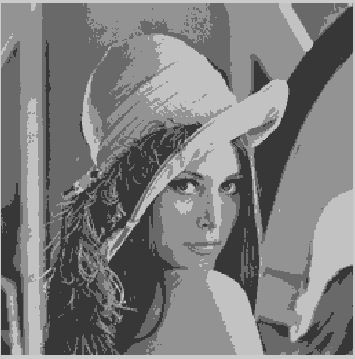
\includegraphics[width=6cm, height=6cm]{../lena_quantlloyd_4_niveaux.jpg}
	\caption{Quantification scalaire optimale de Lloyd-Max, lena.bmp, débit = 2}
	\label{fig:lena_quant_4_niveaux}
\end{figure}

Contrairement à la quantification uniforme, il est possible via cet algorithme de retrouver une distorsion nulle. En effet, les valeurs de reconstruction (niveaux de gris) retrouvées pour un débit égal à 8 sont exactement les mêmes valeurs que pour l'image originale (résultat que nous observons paragraphe \ref{dist_nmse_snr}).

\subsection{Tests sur les différentes images}


\begin{figure}[H]
	\centering
		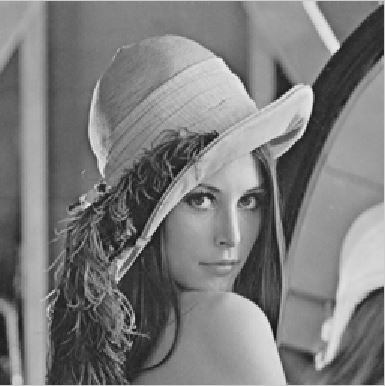
\includegraphics[width=4.5cm, height=4.5cm]{../lena_grey.jpg}
		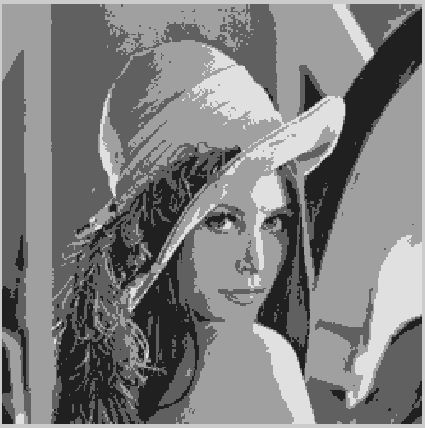
\includegraphics[width=4.5cm, height=4.5cm]{../lena_quant_4_niveaux.jpg}
		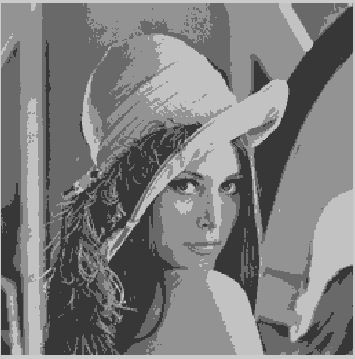
\includegraphics[width=4.5cm, height=4.5cm]{../lena_quantlloyd_4_niveaux.jpg}
	\caption{Comparaison visuelle : (de gauche à droite) image originale en niveaux de gris, image quantifiée uniformément, image quantifiée optimisée selon Lloyd-Max (débit = 4)}
	\label{fig:comparaison_img_quant}
\end{figure}

Nous observons visuellement les différences de qualité entre les deux quantifications mises en oeuvre dans ce TP (avec le même débit). La quantification uniforme apporte un contraste plus important qui vient biaiser les couleurs originales. La quantification scalaire optimale permet de retrouver des couleurs plus fidèles à l'image originale, avec des niveaux de gris moins saillants. En effet, les couleurs retrouvent plus facilement leur appartenance dans les classes qui ont été optimisées selon la densité, ce qui permet de retrouver des couleurs plus fidèles. Mathématiquement, cette qualité est démontrée par la minimisation de l'erreur quadratique que permet l'algorithme de Lloyd-Max :

\begin{table}[!h]
	\centering
		\begin{tabular}{l|c|c|}
			\cline{2-3}
			                               & Lloyd-Max & Uniforme \\
			\hline
			\multicolumn{1}{|l|}{Lena}     & 162.73    &  331.59  \\
			\hline
			\multicolumn{1}{|l|}{Peppers}  & 199.19    &  309.10  \\
			\hline
			\multicolumn{1}{|l|}{Harbour}  & 152.30    &  282.88  \\
			\hline
			\multicolumn{1}{|l|}{Bridge}   & 274.54    &  331.21  \\
			\hline
			\multicolumn{1}{|l|}{Boats}    & 134.59    &  226.24  \\
			\hline
			\multicolumn{1}{|l|}{Airfield} & 285.65    &  405.28  \\
			\hline
		\end{tabular}
	\caption{Comparaison des distorsions - 4 niveaux}
	\label{tab:TableComparaisonDisto}
\end{table}

Des écarts importants sont observés entre les distorsions des deux algorithmes mis en œuvre, pouvant aller du simple au double lorsque les niveaux de reconstruction de la quantification uniforme sont très mal choisis. \\


\subsection{Huffman - Taux de compression des images quantifiées}

Ci-dessous, un tableau récapitulatif des différents taux de compression des images quantifiées puis compressées en utilisant l'algorithme de Huffman.

\begin{table}[H]
	\centering
		\begin{tabular}{l|c | c| c|}
			\cline{2-4}
			                               & Avec Lloyd-Max 4 niveaux & Avec Lloyd-Max 16 niveaux & Sans      \\
			\hline
			\multicolumn{1}{|l|}{Lena}     & 75 \%                    & 52.36 \%                  & 6.66 \%   \\
			\hline
			\multicolumn{1}{|l|}{Peppers}  & 75 \%                    & 51.36 \%                  & 4.77 \%   \\
			\hline
			\multicolumn{1}{|l|}{Harbour}  & 78.15 \%                 & 58.81 \%                  & 15.21 \%  \\
			\hline
			\multicolumn{1}{|l|}{Bridge}   & 75.11 \%                 & 53.14 \%                  & 28.35 \%  \\
			\hline
			\multicolumn{1}{|l|}{Boats}    & 76 \%                    & 54.04 \%                  & 11.74 \%  \\
			\hline
			\multicolumn{1}{|l|}{Airfield} & 75.97 \%                 & 52 \%                     & 10.70 \%  \\
			\hline
		\end{tabular}
	\caption{Taux de compression avec Huffman}
	\label{tab:TableComparaisonTauxCompression}
\end{table}

Évidemment, la compression d'images ayant peu de niveaux de gris est plus efficace, cependant, elle se fait au dépend de la qualité de l'image.

\begin{figure}[H]
	\centering
		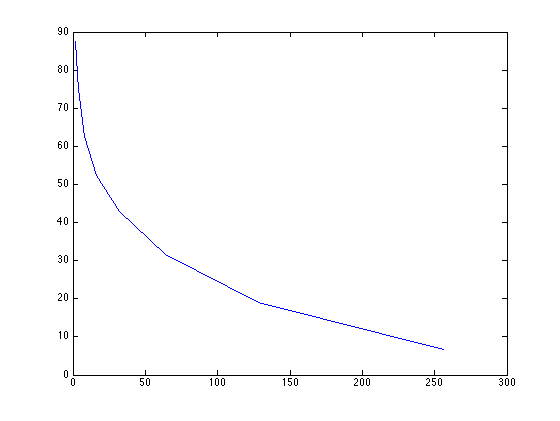
\includegraphics[width=12cm, height=10cm]{../taux_compression_vs_nb_niveaux.png}
	\caption{Taux de compression de lena.bmp en fonction du nombre de niveaux de reconstruction}
	\label{fig:courbe_compression}
\end{figure}

\newpage

\section{Conclusion}

Ce TP nous a permis de se rendre compte de ce qu'implique la quantification. En effet, la distorsion du signal peut-être très importante et la qualité du signal est ainsi dégradée sévèrement. Cependant, nous avons vu qu'avec le même nombre de bits par pixel, il est possible de réduire significativement la distorsion, en appliquant une quantification intelligente qui permet de retrouver des niveaux de reconstruction en moyenne plus proches des valeurs réelles.
De plus, en implémentant l'algorithme de Lloyd-Max, nous avons pu mieux comprendre son fonctionnement.

\clearpage
\appendix

\section{Codes source MATLAB}
\subsection{NMSE et SNR}\label{nmse_snr_code}

\FSource{../disto_1_1.m}

\newpage

\subsection{Quantification uniforme}\label{quant_uni_code}

\FSource{../quant_uni_1_2.m}

\newpage

\subsection{Quantification scalaire optimale de Lloyd-Max}\label{quant_lloyd}

\FSource{../lloyd_max_2_1.m}

\end{document}